\scanpage{373}
\uline{Resolutions canoniques d'un groupe abelien}

\[
X_*(G)\longrightarrow G\qquad X_i(G)=Z(G^n\times\mathbb Z^j)
\]
\diagram{\begin{tikzcd}[column sep=small]
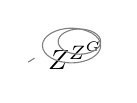
\begin{tikzpicture}[baseline=(z.base)]\node[inner sep=2pt] (z) {$\mathbb Z^{\mathbb Z^G}$};\draw[gray] (.05,.18) ellipse (.27 and .16);\draw[gray] (-.05,.13) ellipse (.37 and .22);\draw[gray] (-.6,-.08)--(-.52,-.03);\end{tikzpicture}\arrow[r,shift left=1ex]\arrow[r]\arrow[r,shift right=1ex] & 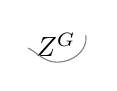
\begin{tikzpicture}[baseline=(z.base)]\node[inner sep=2pt] (z) {$\mathbb Z^G$};\draw[gray] (-.35,-.04) to[out=-30,in=180] (.02,-.22) to[out=0,in=-80] (.38,.12);\end{tikzpicture} & G
\end{tikzcd}}
\[
G\to G!\qquad H
\]
\margin{Pour tout $n$ on a une résolution simpliciale de $K(G,n)$ $\big\}$}
\diagram{\begin{tikzcd}
\mathbb Z^{\mathbb Z K(G,n)}\arrow[r,shift left=1ex]\arrow[r]\arrow[r,shift right=1ex]
&\mathbb Z^{K(G,n)}\arrow[l,shift left=2ex]\arrow[l,shift right=2ex]
\end{tikzcd}}
\[
K(G,n)=G\otimes_{\mathbb Z}\Lambda^n\Psi\qquad n\ \deleted{\text{large}}\ \text{grand}
\]
\[
\begin{aligned}
&r\text{-qis}\quad r<f(n,p)\quad K(\mathbb Z,n)\wedge K(G,p)\xrightarrow{\sim}\mathbb Z(S^n\wedge K(G,p))\longrightarrow\mathbb Z K(G,n+p)\\
&\hspace{7em} S^n\wedge K(G,p)\longrightarrow K(G,n+p).
\end{aligned}
\]
\[
\begin{aligned}
&K(\mathbb Z,p_1)\wedge K(\mathbb Z,p_2)\wedge\cdots\wedge K(\mathbb Z,p_r)\wedge K(G,p_{r+1})\ \sim\quad\mathbb Z^r K(G,\deleted{\unsure{n+}}p)\\
&\sum_{i=1}^{r+1}p_i=p
\end{aligned}
\]
\[
\begin{aligned}
&r\text{ qis}\qquad 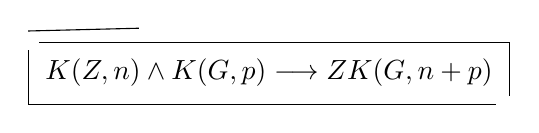
\begin{tikzpicture}[baseline=(b.base)]\node[inner sep=6pt] (b) {$K(\mathbb Z,n)\wedge K(G,p)\longrightarrow\mathbb Z K(G,n+p)$};\draw ([xshift=4pt]b.north west)--(b.north east)--([yshift=3pt]b.south east);\draw ([yshift=-3pt]b.north west)--(b.south west)--([xshift=-5pt]b.south east);\draw ([yshift=4pt]b.north west)--([xshift=40pt,yshift=5pt]b.north west);\end{tikzpicture}\\
&r=\min(n+2p-1,\,2n+p-1)
\end{aligned}
\]
\[
K(\mathbb Z,n)\wedge X\longrightarrow\mathbb Z[S^n\wedge X]
\]
\[
\deleted{K(\mathbb Z,p)\wedge}
\]
\diagram{\begin{tikzcd}[column sep=small]
K(\mathbb Z,n)\wedge K(\mathbb Z,m)\wedge K(\deleted{\mathbb Z}G,p)\arrow[r] & \mathbb Z[S^n\wedge K(\mathbb Z,n)\wedge K(G,p)]\arrow[d]\\
&\mathbb Z[K(\mathbb Z,n+m)\wedge K(G,p)]\arrow[d]\\
&\mathbb Z[\mathbb Z\deleted{\unsure{K}}[S^{n+m}\wedge K(G,p)]]\arrow[d]\\
&\mathbb Z[\mathbb Z K(G,n+m+p)]
\end{tikzcd}}
\mspage{374}
